\RequirePackage{pdfmanagement}
\documentclass[12pt]{article}
\usepackage[letterpaper,top=2cm,bottom=2cm,left=2.54cm,right=2.54cm,marginparwidth=1.75cm]{geometry}
\usepackage{amsmath,amssymb,amsthm,bm}
\usepackage{mathtools}
\usepackage{graphicx}
\usepackage{booktabs}
\usepackage{subcaption}
\DeclareCaptionFont{elevenpt}{\fontsize{11}{13.6}\selectfont}
\captionsetup[figure]{font=elevenpt}
\usepackage{lineno}
\usepackage[colorlinks=true, allcolors=blue]{hyperref}
\usepackage{comment}
\usepackage[dvipsnames]{xcolor}
\usepackage{float}
\usepackage{pgfplots}
\pgfplotsset{compat=1.17}
\usepackage{tikz}
\usetikzlibrary{arrows.meta, positioning, calc}
\usepackage[authoryear,round]{natbib}
\usepackage{standalone}
\usepackage{pdfpages}
\makeatletter\def\input@path{{appendices/}}\makeatother
\usepackage{newpax}
\newpaxsetup{dests/all}
\newtheorem{proposition}{Proposition}
\newtheorem{lemma}{Lemma}
\newtheorem{corollary}{Corollary}
\newtheorem{definition}{Definition}
\newtheorem{remark}{Remark}
\setlength{\parindent}{0pt}
\setlength{\parskip}{6pt plus 2pt minus 1pt}
\makeatletter
\setlength{\@fptop}{0pt}
\setlength{\@fpbot}{0pt plus 1fil}
\renewcommand\section{\@startsection{section}{1}{\z@}{1.5ex plus .5ex minus .2ex}{0.6ex plus .2ex}{\normalfont\Large\bfseries}}
\renewcommand\subsection{\@startsection{subsection}{2}{\z@}{1.0ex plus .3ex minus .2ex}{0.4ex plus .1ex}{\normalfont\large\bfseries}}
\newcommand{\AppendixAMainEquationLink}{%
  \ifnum\AM@page=1\relax
    \setlength{\unitlength}{1bp}%
    \put(75.556,650.865){%
      \hyperref[eq:intro_sigma]{\phantom{\rule{7.845bp}{13.948bp}}}%
    }%
  \fi
}
\newcommand{\AppendixBCrossReferenceLinks}{%
  \ifnum\AM@page=1\relax
    \setlength{\unitlength}{1bp}%
    \put(236.870,573.465){%
      \hyperlink{appendixA.1}{\phantom{\rule{64.865bp}{12.619bp}}}%
    }%
    \put(229.304,455.230){%
      \hyperlink{appendixA.1}{\phantom{\rule{20.523bp}{13.948bp}}}%
    }%
  \fi
  \ifnum\AM@page=4\relax
    \setlength{\unitlength}{1bp}%
    \put(378.549,463.228){%
      \hyperlink{appendixA.5}{\phantom{\rule{26.376bp}{13.947bp}}}%
    }%
  \fi
}
\makeatother
\renewenvironment{abstract}{%
  \noindent{\bfseries \abstractname}\par\vspace{-4pt}\noindent\ignorespaces
}{}
% --- notation shorthands ---
\newcommand{\R}{\mathbb{R}}
\newcommand{\C}{\mathbb{C}}
\newcommand{\vech}{\operatorname{vech}}
\newcommand{\vc}{\operatorname{vec}}
\newcommand{\tr}{\operatorname{tr}}
\newcommand{\Real}{\operatorname{Re}}
\newcommand{\Imag}{\operatorname{Im}}
\newcommand{\Lop}{\mathcal{L}}
\newcommand{\Mbf}{\mathbf{M}}
\newcommand{\Kbf}{\mathbf{K}}
\newcommand{\E}{\mathbb{E}}
\DeclareMathOperator{\atantwo}{atan2}
\newcommand{\adj}{\operatorname{adj}}
\title{A triple-operator decomposition of a map from causal to correlational brain connectivity at rest: intrinsic dynamics, temporal coloring, and spatial covariance}
\author{Yaohui Ding}
\begin{document}
\setcounter{secnumdepth}{-1}
\maketitle
\linenumbers 
% ======================================================================
\begin{abstract}
Correlational brain connectivity, roughly speaking, tells us how the activity from different brain regions covary. Causal brain connectivity, on the other hand, describes how different brain regions causally influence each other. Both types of brain connectivity at rest are commonly used for psychiatric classification in research settings, which is an important goal in computational psychiatry. Spectral dynamic causal modeling (DCM) is a widely used framework for inferring causal brain connectivity from resting state functional magnetic resonance imaging data. Crucially, spectral DCM entiles a deterministic map from causal to correlational brain connectivity, which can be expressed as a matrix-valued complex integral in the frequency domain. In the current study, we solve this matrix-valued integral and derive an analytic formula linking causal and correlational (more precisely covariance) patterns of brain connectivity. We show that this formula satisfies a Lyapunov equation with causal connectivity-dependent forcing, which is also the symmetrized zero-lag state--noise cross-covariance. Finally, we show that the steady-state covariance can be decomposed into three multiplicative factors (or operators) that have distinct roles, namely intrinsic neuronal dynamics (mean reversion), connectivity-dependent temporal coloring (scale-free), and a spatial covariance operator. Together, these results turn the deterministic relationship between causal and correlational brain connectivity in the frequency domain into a transparent algebraic formula that explains how intrinsic neuronal dynamics and the temporal and spatial characteristics of noise fluctuation jointly shape the correlational patterns of brain activity at rest.
\end{abstract}
\par\smallskip
\noindent\textbf{Keywords:} resting state brain connectivity; spectral dynamic causal modeling; Lyapunov equation; colored noise
% ======================================================================
\section{Introduction}
\label{sec:intro}
\subsection{Psychiatric classification with brain connectivity at rest}
\label{sec:intro_motivation}
Correlational and causal patterns of brain connectivity at rest carry different kinds of information about a brain network of interest. Metrics of correlational brain connectivity are generally symmetric and are summary statistics of measured brain activity, whereas metrics of causal connectivity describe directed interactions among a set of brain regions and are infered from observed brain activity \citep{Friston2011}. 
Both types of brain connectivity are commonly utilized for psychiatric classification. For example patterns of correlation among regional blood oxygenation-level dependent (BOLD) signals, termed resting-state functional connectivity, have been used to define subtypes of depression \citep{Drysdale2017RestingStateBiotypes}. Model-based estimates of causal connectivity among different brain regions at rest, termed resting-state effective connectivity, have also served as features for classifying and predicting future depressive episodes \citep{Galioulline2023}. 

\subsection{The current study}
\label{sec:intro_prior_current}
\textbf{Motivation.} The current study is motivated by the lack of an explicit analytic formula linking causal (or effective) and correlational (or functional) patterns of brain connectivity at rest, when the casual connectivity is \textit{asymmetric} and the neuronal noise fluctuation is both temporally- and \textit{spatially-correlated}. Such an analytic relationship can help explain how directed causal brain connectivity gives rise to symmetric correlational brain connectivity. It can also provide a common mathematical framework for interpreting results from empirical studies of resting state causal and correlational brain connectivity, as defined in the spectral dynamic causal modeling (DCM) framework \citep{Friston2014}. An analytic formula relating resting state correlational to causal connectivity is derived in \citet{FristonNodesModes2014}, but with assumptions of \textit{symmetric} effective connectivity and \textit{spatially-independent} noise fluctuations.


\textbf{Contributions.} \textit{First}, we derive an explicit analytic formula for general $n \times n$ causal networks with temporally- and spatially-correlated noise fluctuations. \textit{Second}, we prove that the covariance formula satisfies a Lyapunov equation with connectivity-dependent forcing and identify that forcing as the symmetrized zero-lag state--noise cross-covariance. \textit{Third}, we show that the map from causal to correlational (more precisely covariance) patterns of brain connectivity at rest can be decomposed into three operators, namely, intrinsic dynamics, connectivity-dependent temporal coloring, and a spatial covariance operator.

\section{Methods}
\subsection{The generative model of spectral dynamic causal modeling}
\label{sec:intro_sdcm}
Spectral DCM models the cross-spectral density of resting-state BOLD signals \citep{Friston2014,FristonNodesModes2014,Razi2015} and has two levels. Neuronal activity $\boldsymbol{x}(t)\in\mathbb{R}^{n}$ of $n$ regions evolves linearly under stochastic drive,
\begin{equation}
\dot{\boldsymbol{x}}(t)=\mathbf{A}\,\boldsymbol{x}(t)+\boldsymbol{w}(t),
\label{eq:intro_sde}
\end{equation}
where $\mathbf{A}$ is the effective-connectivity matrix and $\boldsymbol{w}(t)$ is neuronal noise.
The observed BOLD signal is
\begin{equation}
\boldsymbol{y}(t)=\mathbf{H}\,\boldsymbol{x}(t)+\boldsymbol{e}(t),
\label{eq:intro_obs}
\end{equation}
where $\mathbf{H}$ is an invertible but frequency-dependent matrix that models the hemodynamic response and $\boldsymbol{e}(t)$ is observation noise. To focus on neuronal covariance, we set $\mathbf H=\mathbf I$ and the observation noise to zero ($\mathbf e(t)=\mathbf 0$), so that $\boldsymbol y(t)=\boldsymbol x(t)$. In spectral DCM, the neuronal noise $\mathbf w(t)$ is modeled as a stationary, zero-mean multivariate Gaussian generalized process with the idealized power-law spectrum
\begin{equation}
\mathbf{S}_w(\omega)=\alpha\,|\omega|^{-\beta}\,\boldsymbol{\Sigma}_w,
\qquad -1<\beta<1,
\label{eq:intro_Sw}
\end{equation}
where $\boldsymbol\Sigma_w$ is a real symmetric positive-semidefinite spatial covariance factor. Setting $\beta=0$ leads to the more conventional white noise assumption and larger $\beta$ concentrates power at lower frequencies. With $\mathbf R(\omega):=(i\omega\mathbf I-\mathbf A)^{-1}$, the cross-spectral density of $\boldsymbol y$ is \citep[][Eq.~22]{Novelli2024}
\begin{equation}
\mathbf{G}_y(\omega)
=\mathbf R(\omega)\,\mathbf S_w(\omega)\,\mathbf R(\omega)^\dagger.
\label{eq:intro_Gy}
\end{equation}
Substituting \eqref{eq:intro_Sw} into \eqref{eq:intro_Gy} and integrating over frequency gives \citep[][Eq.~37]{Novelli2024}
\begin{equation}
\boldsymbol{\Sigma}(\mathbf{A},\alpha,\beta,\boldsymbol\Sigma_w)
:=\frac{1}{2\pi}\int_{-\infty}^{\infty}\mathbf{G}_y(\omega)\,d\omega
=\frac{\alpha}{2\pi}\int_{-\infty}^{\infty}|\omega|^{-\beta}\,
\mathbf R(\omega)\boldsymbol\Sigma_w\mathbf R(\omega)^\dagger\,d\omega.
\label{eq:intro_sigma}
\end{equation}
Spectral DCM thus entails a deterministic map $F:\mathbf{A}\mapsto\boldsymbol{\Sigma}(\mathbf{A},\beta)$ in the frequency domain (Figure~\ref{fig:spectral_dcm_schematic}).

\begin{figure}[H]
\centering
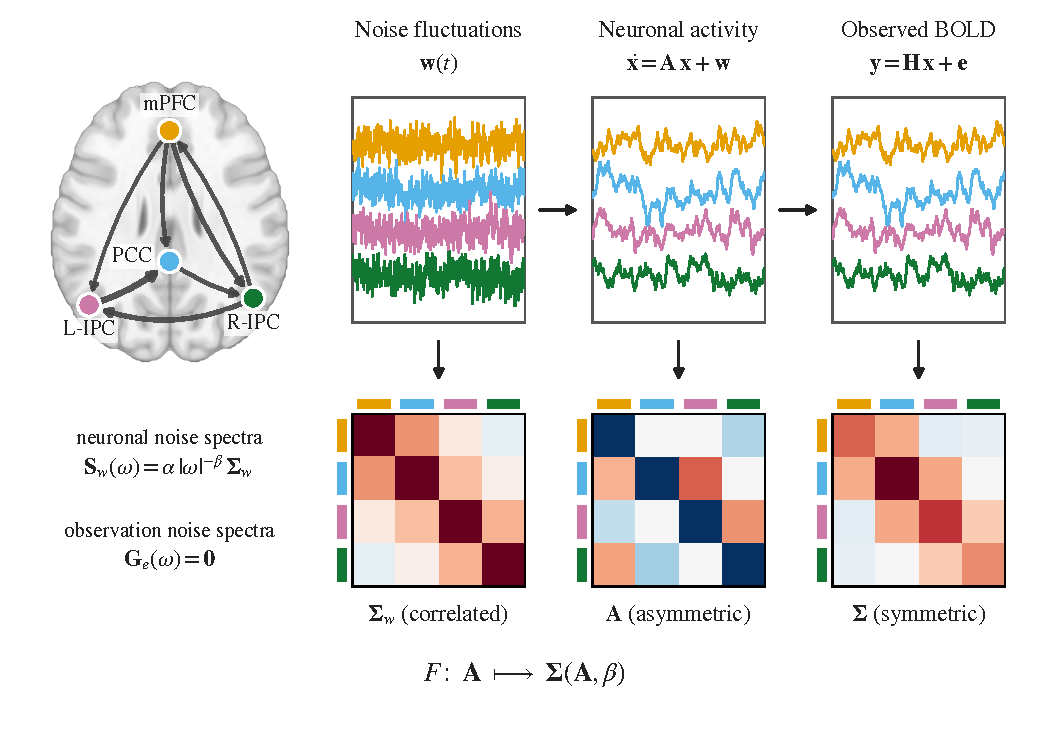
\includegraphics[width=\linewidth,trim=18bp 9bp 15bp 2bp,clip,keepaspectratio]{figures/spectral_dcm_schematic/spectral_dcm_schematic.pdf}
\caption{\textbf{A schematic of the generative model in spectral dynamic causal modeling in \cite{Friston2014}}. We use four default-mode regions (mPFC, PCC, L-IPC, and R-IPC) to illustrate a directed network. Thicker arrows indicate stronger causal influences. The matrix panels contrast a nondiagonal spatial covariance factor, asymmetric causal connectivity, and symmetric covariance. Colored bars identify regions. All parameter values are picked illustrative purposes. The observation mapping is set to the identity matrix. Neuronal noise has unit amplitude, unit marginal spatial variance, and a power-law exponent of 0.5, and observation noise is set to zero.}
\label{fig:spectral_dcm_schematic}
\end{figure}
\vspace{-8pt}

\subsection{Techniques}
Here we briefly describe the key techniques that we employ in \hyperlink{appendixA}{Appendix A} and \hyperlink{appendixB}{Appendix B} to solve the matrix-valued integral in equation \ref{eq:intro_sigma} and to derive the results in our study. 

\textbf{Parity.} The first insight is to realize the matrix-valued integral can be decomposed into a series of scalar integrals through a pairty argument, i.e., the part of the integrand that is multiplied by the imaginary variable ($i$) is odd, see \hyperlink{appendixA.3}{Appendix~A, Eq.~(A-17)} and \hyperlink{appendixB.3}{Appendix~B, Eq.~(B-20)}. Hence, it is evaluated to zero. Hurwitz stability
and $-1<\beta<1$ ensure absolute convergence of the other terms that are left in the integrand. 

\textbf{Euler's beta integral.} Partial fraction reduce the scalar integral to the evaluation of
$I_\beta(c):=\int_{\mathbb R}|\omega|^{-\beta}/(\omega^2+c^2)\,d\omega$.
For real $c<0$, this integral can be transformed to Euler's beta integral through a change of variables
(\hyperlink{appendixA.4}{Appendix~A, Eqs.~(A-26)--(A-31)}), yielding the
closed-form solution in \hyperlink{appendixA.5}{Eq.~(A-32)}.

\textbf{Analytic continuation.} To admit complex
eigenvalues, we use an analytic continuation argument in \hyperlink{appendixA.4}{Appendix~A} to show the closed-form solution of \hyperlink{appendixA.5}{Eq.~(A-32)} also applies to complex eigenvalues, i.e., $\operatorname{Re}c<0$.

\textbf{Eigen-decomposition.} For a diagonalizable $n\times n$ network, we write
$\mathbf A=\mathbf P\boldsymbol\Lambda\mathbf P^{-1}$ and factor both
resolvents in this eigenbasis. With
$\mathbf M_w=\mathbf P^{-1}\boldsymbol\Sigma_w\mathbf P^{-\dagger}$, the
diagonal resolvents turn the matrix integral into an entrywise product
(\hyperlink{appendixB.3}{Appendix~B, Eq.~(B-17)}), and every entry reduces to
two evaluations of the same $I_\beta$
(\hyperlink{appendixB.4}{Eqs.~(B-23)--(B-26)}).

\textbf{Lyapunov operator.} To show the covariance formula in equation (\ref{eq:results_general_covariance}) satisfies a Lyapunov equation, we first define a Lyapunov operator in the eigenbasis of $\mathbf A$, i.e., $\mathbf P (\mathbf A \boldsymbol{\Sigma} + \boldsymbol{\Sigma} \mathbf A^{T}) \mathbf P^{\dagger}$. Next, through a series of algebraic steps, we show it leads to a Lyapunov equation in this eigenbasis, which is then transformed back to the original basis-free coordinates, see \hyperlink{appendixB.6}{Appendix~B, Eqs.~(B-30)--(B-38)}. Finally, we use a combination of vectorization and Kronecker product techniques to solve the Lyapunov equation, leading to the factorized
solution in \hyperlink{appendixB.7}{Eqs.~(B-43)--(B-48)}.

\subsection{AI Use Disclosure}
Large language models (LLMs) were used to help with some steps of the derivation in \hyperlink{appendixA}{Appendix A} and \hyperlink{appendixB}{Appendix B}. LMMs were also used for preparing the manuscript. Use of these AI tools were under the author's iterative guidance, supervision, and revision. Finally, the author is solely responsible for the mathematical derivations, results, interpretations, and conclusions presented in the current manuscript.
% ======================================================================
\section{Results}\label{sec:results}
\subsection{The covariance formula for dyadic interaction}
\label{sec:results_dyad}

The following results are derived in
\hyperlink{appendixA.7}{Appendix~A}. The formula for the stationary neuronal covariance (\hyperlink{appendixA.7}{Appendix~A, Eq.~(A-40)}) is
\begin{equation}
    \boldsymbol{\Sigma}
    =\frac{\alpha}{2\tr(\mathbf{A})\cos(\pi\beta/2)}
    \Bigl[f\,\boldsymbol\Sigma_w+g\,\adj(\mathbf{A})\boldsymbol\Sigma_w\adj(\mathbf{A})^\top\Bigr],
    \label{eq:results_dyadic_covariance}
\end{equation}
Here $\adj(\mathbf A)$ denotes the adjugate of $\mathbf A$. The first line below applies to distinct
eigenvalues and the second gives the continuous limit at
$\lambda_1=\lambda_2=a$:
\begin{equation}
\begin{aligned}
    f&:=\frac{(-\lambda_2)^{1-\beta}-(-\lambda_1)^{1-\beta}}{\lambda_2-\lambda_1},
    &\qquad
    g&:=\frac{(-\lambda_1)^{-1-\beta}-(-\lambda_2)^{-1-\beta}}{\lambda_2-\lambda_1},
    \\
    f&:=-(1-\beta)(-a)^{-\beta},
    &\qquad
    g&:=-(1+\beta)(-a)^{-2-\beta}.
\end{aligned}
    \label{eq:results_dyadic_coefficients}
\end{equation}

Writing $a=\tr(\mathbf A)/2$, the eigenvalues are
\begin{equation}
\begin{aligned}
    \lambda_1&=a-\sqrt{a^2-\det\mathbf A},
    &\qquad
    \lambda_2&=a+\sqrt{a^2-\det\mathbf A}.
\end{aligned}
    \label{eq:results_dyadic_lambda_one}
\end{equation}


\subsection{The covariance formula for $n\times n$ networks}
\label{sec:results_nbyn_network}
The covariance formula for general $n\times n$ network is derived in
\hyperlink{appendixB.5}{Appendix~B, Eq.~(B-28)}. For a diagonalizable $A$ matrix, we write
$\mathbf A=\mathbf P\boldsymbol\Lambda\mathbf P^{-1}$, with eigenvalues
$\lambda_k$ on the diagonal of $\boldsymbol\Lambda$. The formula for the steady state covariance is, 
\begin{equation}
    \boldsymbol{\Sigma}(\mathbf{A},\beta)=\eta_\beta\,\mathbf{P}\,
    \Bigl[(M_w)_{kl}\,
    \frac{(-\lambda_k)^{-\beta}+(-\bar\lambda_l)^{-\beta}}
    {-(\lambda_k+\bar\lambda_l)}\Bigr]_{k,l=1}^{n}\,\mathbf{P}^{\dagger},
    \label{eq:results_general_covariance}
\end{equation}

where $[x_{kl}]_{k,l=1}^n$ denotes the $n\times n$ matrix with entries $x_{kl}$, and 
\begin{equation}
\begin{aligned}
    \eta_\beta:=\frac{\alpha}{2\cos(\pi\beta/2)},
    &\qquad
    \mathbf M_w:=\mathbf P^{-1}\boldsymbol\Sigma_w\mathbf P^{-\dagger}
\end{aligned}
    \label{eq:eta_beta}
\end{equation}


\subsection{The covariance formula satisfies a Lyapunov equation}
\label{sec:results_lyapunov}
We show that the covariance formula in (Eq.~\ref{eq:results_general_covariance})
satisfies a Lyapunov equation (\hyperlink{appendixB.6}{Appendix~B, Eq.~(B-38)}),
\begin{equation}
\mathbf{A}\boldsymbol{\Sigma}+\boldsymbol{\Sigma}\mathbf{A}^\top
    +\eta_\beta\Bigl[(-\mathbf{A})^{-\beta}\boldsymbol{\Sigma}_w
    +\boldsymbol{\Sigma}_w\bigl[(-\mathbf{A})^{-\beta}\bigr]^{\top}\Bigr]
    =\mathbf{0}.
    \label{eq:results_lyapunov_colored}
\end{equation}
Equivalently, this is a continuous-time Lyapunov equation (\hyperlink{appendixB.6}{Appendix~B, Eq.~(B-40)}),
\begin{equation}
\mathbf A\boldsymbol\Sigma+\boldsymbol\Sigma\mathbf A^\top+
\mathbf Q_\beta(\mathbf A,\boldsymbol\Sigma_w)=\mathbf0,
\label{eq:results_lyapunov_standard}
\end{equation}

where
\begin{equation}
\mathbf Q_\beta(\mathbf A,\boldsymbol\Sigma_w)
:=\eta_\beta[(-\mathbf A)^{-\beta}\boldsymbol\Sigma_w+
\boldsymbol\Sigma_w[(-\mathbf A)^{-\beta}]^\top].
\label{eq:Q_beta}
\end{equation}

Furthermore,  we show that $\eta_\beta(-\mathbf A)^{-\beta}\boldsymbol{\Sigma}_w$ is the zero-lag state--noise cross-covariance
$\boldsymbol\Sigma_{xw}$ (\hyperlink{appendixB.6}{Appendix~B, Eq.~(B-59)}), i.e.,
\begin{equation}
    \boldsymbol{\Sigma}_{xw}
    =\eta_\beta(-\mathbf A)^{-\beta}\boldsymbol{\Sigma}_w.
    \label{eq:results_cross_covariance}
\end{equation}
Therefore, the Lyapunov equation in Eq.~(\ref{eq:results_lyapunov_colored}) can be written equivalently as (\hyperlink{appendixB.6}{Appendix~B, Eq.~(B-60)})
\begin{equation}
    \mathbf A\boldsymbol{\Sigma}+\boldsymbol{\Sigma}\mathbf A^\top
    +\boldsymbol{\Sigma}_{xw}+\boldsymbol{\Sigma}_{xw}^{\top}
    =\mathbf 0 .
    \label{eq:results_cross_covariance_balance}
\end{equation}

\subsection{A triple-operator decomposition of steady state covariance}
\label{sec:results_lyapunov}
Finally, we decompose the solution to equation (\ref{eq:results_lyapunov_colored}) into three operators, using standard vectorization and Kronecker product techniques, where $\vc(\cdot)$ denotes column-stacking vectorization and
$\otimes$ the Kronecker product. Hurwitz  stability guarantees the Kronecker sum ($\mathbf I\otimes\mathbf A+\mathbf A\otimes\mathbf I$) is always invertible. 
\begin{equation}
\vc(\boldsymbol\Sigma)
={}
\underbrace{-\bigl(\mathbf I\otimes\mathbf A+\mathbf A\otimes\mathbf I\bigr)^{-1}}
_{\mathcal P_{\mathbf A}}
\underbrace{\left\{\eta_\beta\bigl[\mathbf I\otimes(-\mathbf A)^{-\beta}
+(-\mathbf A)^{-\beta}\otimes\mathbf I\bigr]\right\}}
_{\mathcal T_{\beta,\mathbf A}}
\underbrace{\vc(\boldsymbol\Sigma_w)}
_{\mathbf v_w},
\label{eq:results_vectorized_lyapunov}
\end{equation}
where
\begin{equation*}
\begin{aligned}
\mathcal P_{\mathbf A}&:\quad \text{intrinsic dynamics (mean reversion)},\\
\mathcal T_{\beta,\mathbf A}&:\quad \text{connectivity-dependent temporal coloring (scale-free)},\\
\mathbf v_w&:\quad \text{spatial covariance structure (multivariate Gaussian in Eq.~}\eqref{eq:intro_Sw}\text{)}.
\end{aligned}
\end{equation*}


\section{Discussion}
\label{sec:discussion}
\subsection{Steady-state covariance expressed in the eigenmodes of effective connectivity}
A close examination of the formula in equation~\eqref{eq:results_general_covariance} reveals that the steady state covariance matrix ($\boldsymbol\Sigma=\mathbf P[\cdots]\mathbf P^\dagger$) and the effective connectivity matrix ($\mathbf A=\mathbf P \boldsymbol\Lambda \mathbf P^{-1}$) share the same right eigenmodes (columns of $\mathbf P$). They share the same eigenmodes when $\mathbf A$ is symmetric and the spatial covariance operator is diagonal and isotropic ($\boldsymbol\Sigma_w=\sigma \boldsymbol{I}$). This is because, the eigenvectors of $\mathbf A$ can be chosen in a way such that they form a real and orthonormal matrix, i.e., $\mathbf P^{-1}=\mathbf P^{T}=\mathbf P^{\dagger} $ and $\mathbf P \mathbf P^{\dagger}=\mathbf P^{\dagger} \mathbf P =\boldsymbol{I}$. Therefore, $\mathbf M_w=\mathbf P^{-1}\boldsymbol{\Sigma_w}\mathbf P^{-\dagger}=\boldsymbol{\Sigma_w} (\mathbf P^{-1}\mathbf P^{-\dagger})=\boldsymbol{\Sigma_w} (\mathbf P^{\dagger} \mathbf P)^{-1}=\sigma \boldsymbol{I}$. Each eigenvalue of $\boldsymbol\Sigma$ is a nonlinear functions of $\alpha$, $\beta$, and a pair of eigenvalues from $\mathbf A$ (one of them conjugated; e.g., $\lambda_k$ and $-\bar\lambda_l$). These agree with the main results that are proven in \citet{FristonNodesModes2014}, which assumes symmetric effective connectivity
and spatially independent and equal-variance noise fluctuations. The formula from our study (Eq.~\ref{eq:results_general_covariance}) generalizes their result to asymmetric, Hurwitz-stable
$\mathbf A$ and spatially correlated covariance factor $\boldsymbol\Sigma_w$.

\subsection{A Lyapunov equation with connectivity-dependent forcing}
Equation~\eqref{eq:results_lyapunov_standard} shows that the steady-state covariance solves a continuous-time Lyapunov equation. For fixed $\mathbf A$, $\beta$, and $\boldsymbol\Sigma_w$, it is linear in the unknown $\boldsymbol\Sigma$ and has a unique solution when $\mathbf A$ is Hurwitz stable. Unlike the white noise ($\beta=0$) scenario, the forcing term $\mathbf Q_\beta(\mathbf A, \boldsymbol\Sigma_w)$ in our case, however, depends on a fractional matrix power of the effective connectivity ($(-\mathbf{A})^{-\beta}$). This shows that the effect of temporally-correlated noise is connectivity-dependent. Additionally, equations \eqref{eq:results_cross_covariance} and \eqref{eq:results_cross_covariance_balance} show that the forcing can also be interpreted as symmetrized state-noise cross-covariance($\boldsymbol\Sigma_{xw}+{\boldsymbol\Sigma^T_{xw}}$) at zero-lag. At $\beta=0$, the matrix power becomes the identity and the symmetrized cross-covariance reduces to $\alpha\boldsymbol\Sigma_w$, recovering the standard Lyapunov equation with white-noise forcing.


\subsection{The spatial and temporal characteristics of noise fluctuation play distinct roles in shaping steady-state covariance}
The major contribution of the current study is a triple-operator decomposition of the neuronal covariance at steady-state. \citet{Novelli2024} formulates the map ($F:\mathbf{A}\mapsto\boldsymbol\Sigma$) as a matrix-valued complex integral in the frequency domain. We obtained an analytic closed-form solution to this integral in closed-form, while relaxing their assumption of spatially independent neuronal fluctuations. In so doing, we show that the vectorized covariance in Eq.~\eqref{eq:results_vectorized_lyapunov} can be decomposed into three multiplicative operators with distinct roles,
\begin{equation*}
\vc(\boldsymbol\Sigma)=\mathcal P_{\mathbf A}\,
\mathcal T_{\beta,\mathbf A}\,\mathbf v_w.
\end{equation*}
Here $\mathcal P_{\mathbf A}$ denotes the propagation of the intrinsic neuronal dynamics (mean-reverting). The operator $\mathcal T_{\beta,\mathbf A}$ describes connectivity-dependent, scale-free temporal coloring, whereas $\mathbf v_w$ specifies the spatial covariance structure of the neuronal noise. This decomposition suggests the spatial covariance vector is first transformed by the temporal-coloring
operator and then propagated through the inverse Lyapunov operator associated with mean reversion.

\subsection{Limitations and future directions}
The current study assumes linear time-invariant neuronal dynamics with a
Hurwitz-stable and diagonalizable effective-connectivity matrix, an idealized power-law spectrum over all frequencies, and---to isolate neuronal covariance---an identity observation map ($\mathbf H=\mathbf I$) with no observation noise. However, we note that nondiagonalizable (defective) Hurwitz-stable matrices form a measure-zero subset of the stable matrices \citep{HornJohnson2013,Mityagin2020ZeroSet}. Exact power laws over the entire frequency axis are idealizations. Band-limited or regularized spectra would be more physiologically realistic. Likewise, though more realistic, a frequency-dependent hemodynamic response ($\mathbf H(\omega)$) complicates the mapping from neuronal covariance to the covariance of observed BOLD signals. Nevertheless, we show in \hyperlink{appendixB.7}{Appendix~B, Eq.~(B-72)} that our results generalize to networks with region-specific power-law exponent. Thus, future work should assess how finite frequency cutoffs, frequency-dependent hemodynamics, and observation noise may modify the covariance formulae and their potential Lyapunov representations.  


% ======================================================================
\section*{Code Availability}
No experimental or simulated data are analyzed in the current study. All code necessary to reproduce the manuscript is publicly available at \url{https://github.com/yaohuiding1/corr_causation_map_decomposition}.

%======================================================================

\section*{Acknowledgments}
The author would like to thank John J.B. Allen, Jessica Andrews-Hanna, and Ying-hui Chou for inspiring his curiosity and interest in the topic of causal modeling of brain connectivity at rest. The author would also like to acknowledge John Pearson, Kevin Kuper, Miles Martinez, and Siyu Wang for helpful discussions on the topic of causal modeling of dynamical systems in general.
% ======================================================================
\section{Conflict of Interest}
The author declares no conflict of interest.

% TODO: add competing-interests statement.
% Appendix-only citations: not cited in the main text but needed in bibcites.tex so the appendices resolve them.

\nocite{HornJohnson2013,Folland1999,SteinShakarchi2003,Higham2008,Pavliotis2014,Marquardt2007MFICARMA} 

\bibliographystyle{plainnat}
\bibliography{corr_causation_map_decomposition}
% ======================================================================
%\clearpage
%\includepdf[pages=-,link,linkname=appendixA,pagecommand={\thispagestyle{plain}}]{appendices/build/appendix_a_systematic_review.pdf}

\clearpage
\newpaxsetup{destsuffix=A}
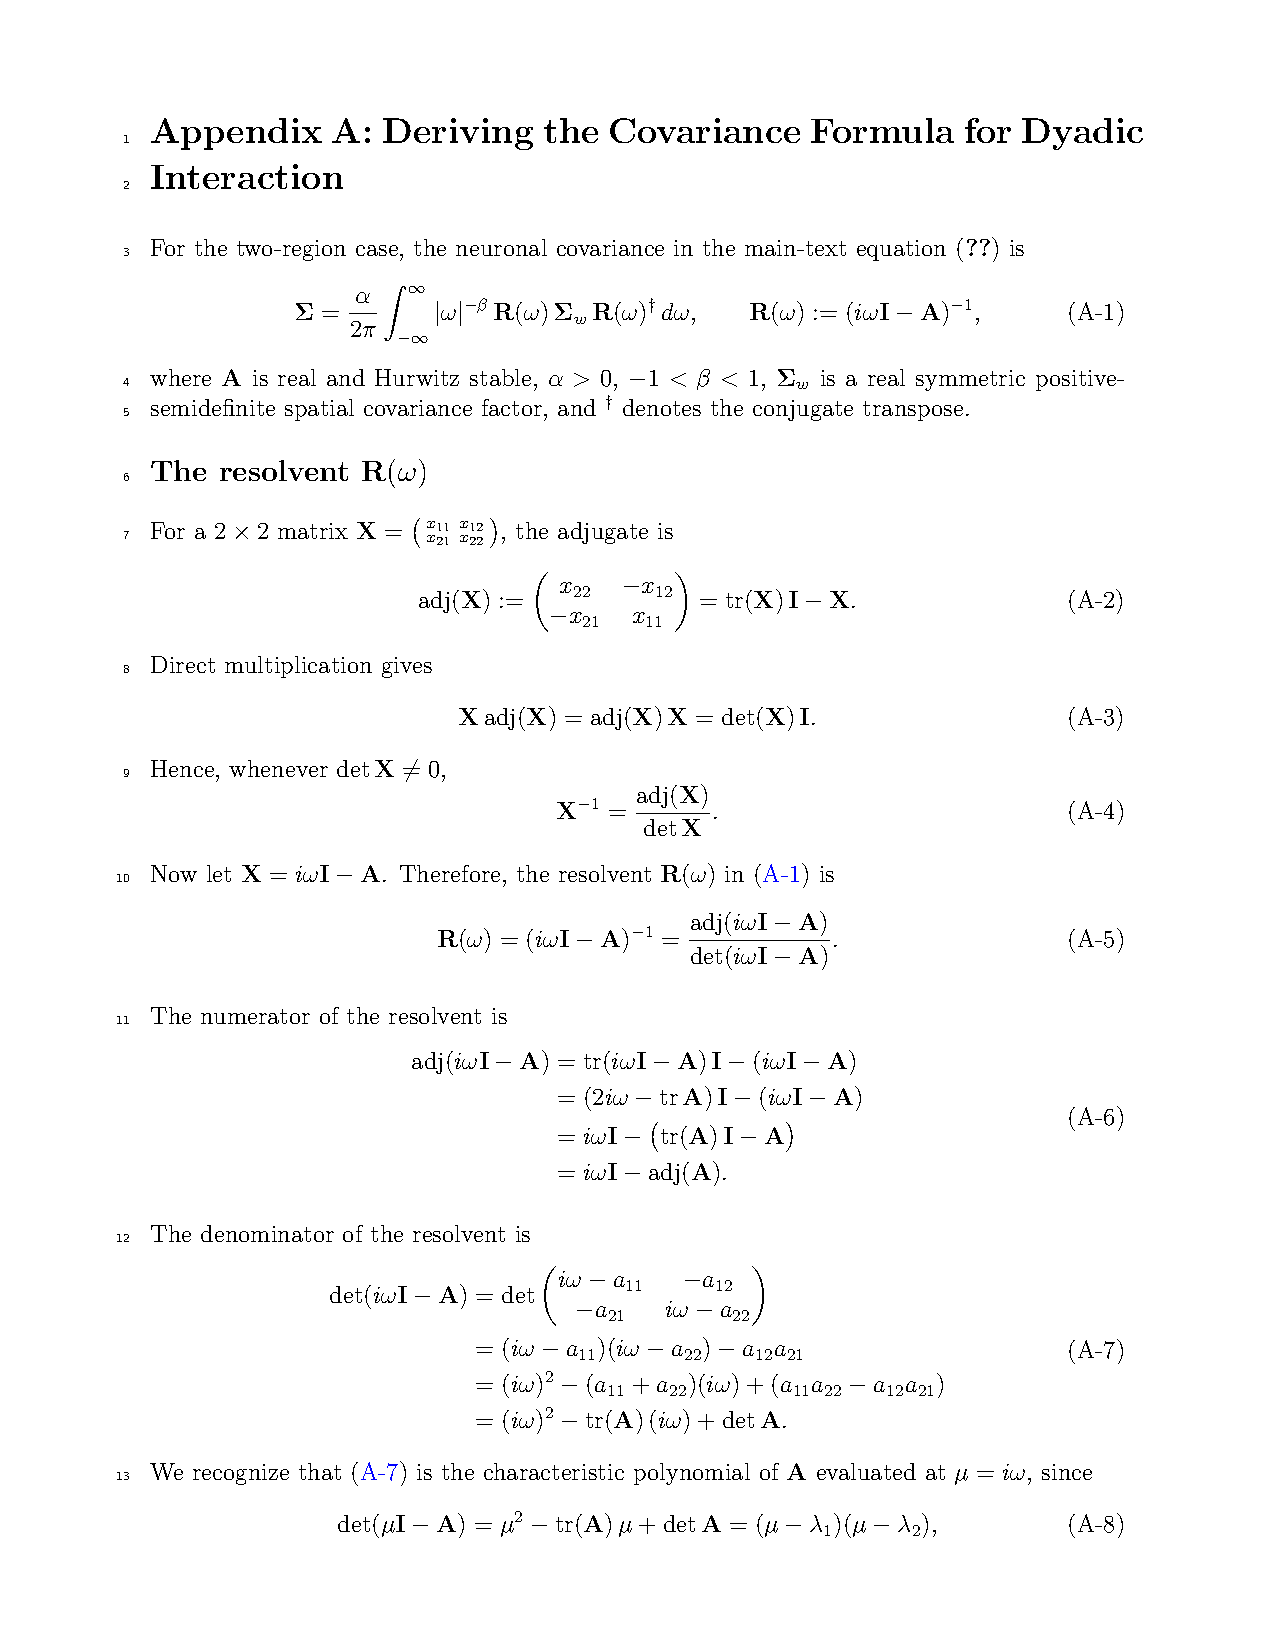
\includepdf[pages=-,link,linkname=appendixA,pagecommand={\thispagestyle{plain}},picturecommand={\AppendixAMainEquationLink}]{appendices/build/appendix_a_cov_formula_dyad.pdf}

\clearpage
\newpaxsetup{destsuffix=B}
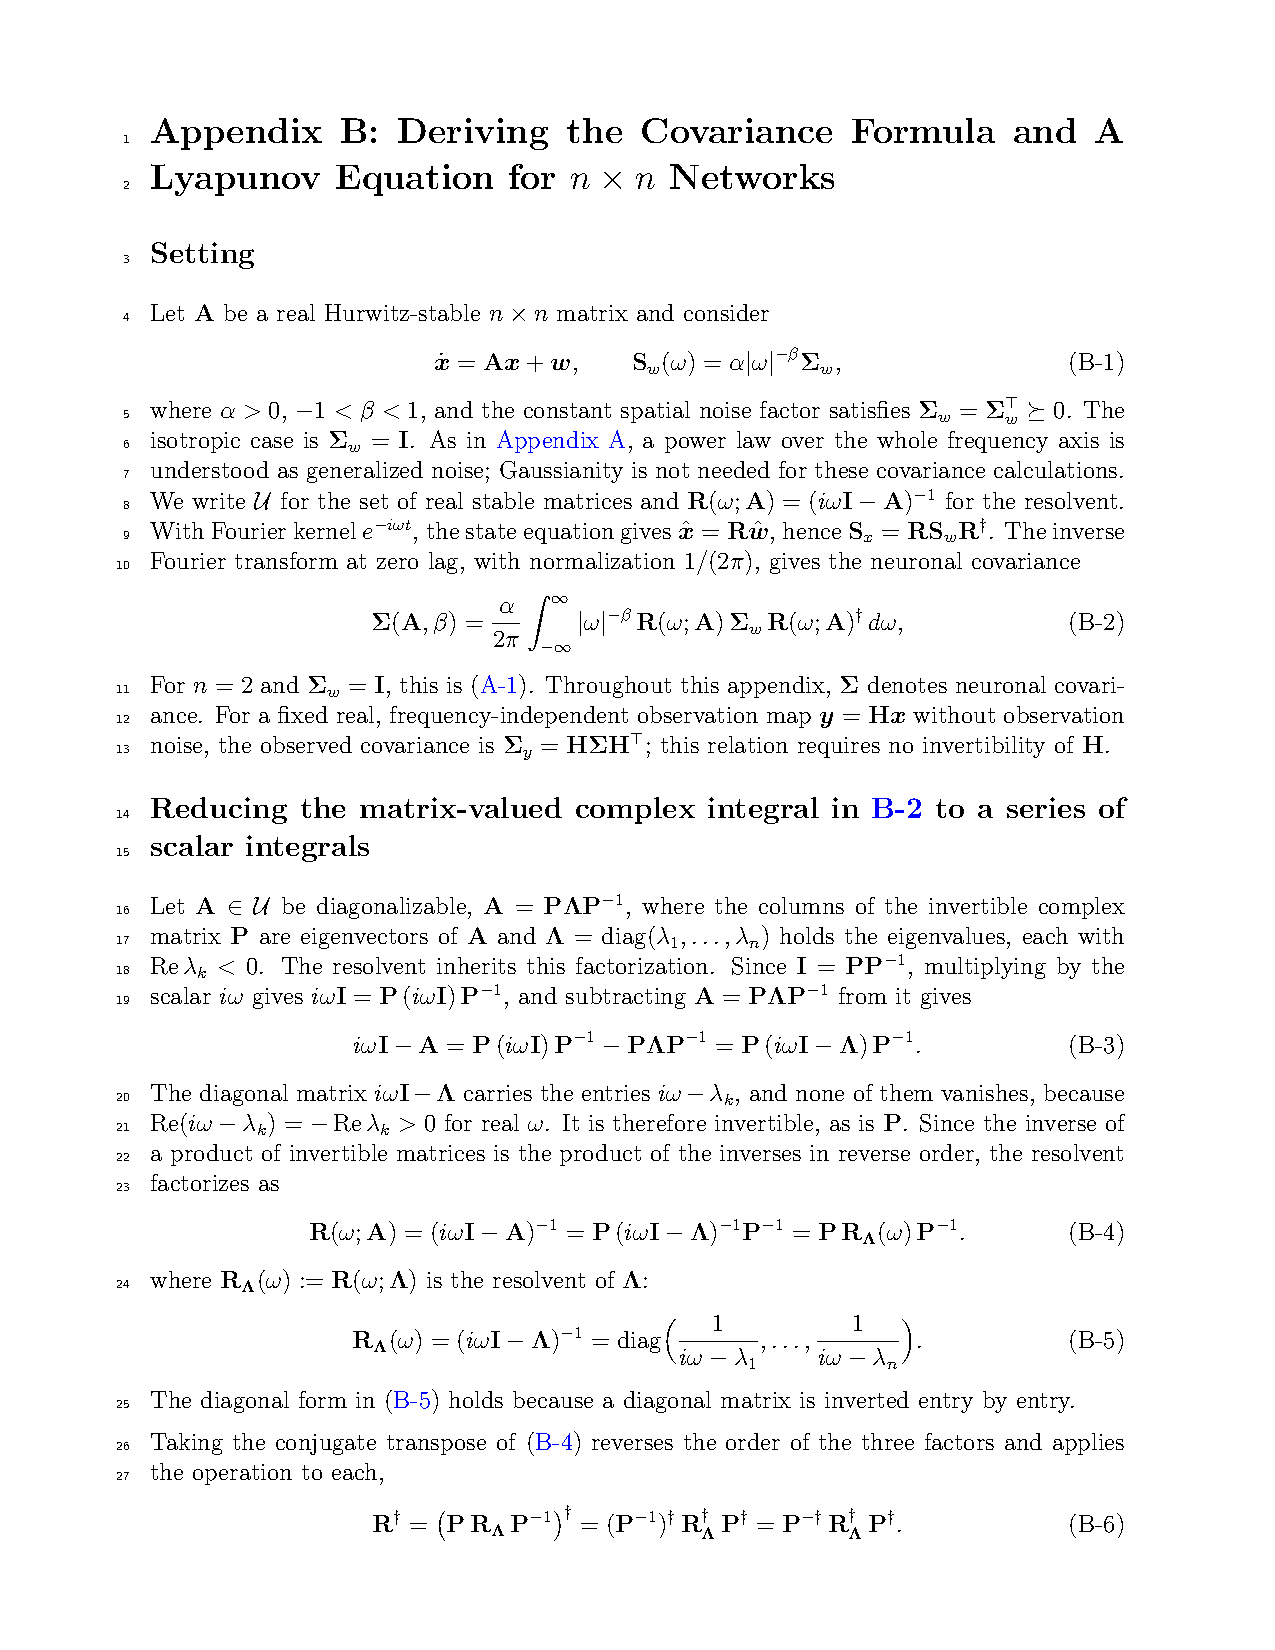
\includepdf[pages=-,link,linkname=appendixB,pagecommand={\thispagestyle{plain}},picturecommand={\AppendixBCrossReferenceLinks}]{appendices/build/appendix_b_cov_formula_nbyn_lyapunov.pdf}


\end{document}
